\chapter{Motivation}\label{chap:motivation}
\setlength\epigraphwidth{.6\textwidth}
\epigraph{That very night in Max's room a forest grew\\
and grew--\\
and grew until his ceiling hung with vines\\
and the walls became the world all around}{---Maurice Sendak,
\emph{Where the Wild Things Are}}


One of the most fascinating things about knot theory is the disconnect
between the relative ease of posing a question and the great
difficulty of providing a rigorous answer to it. Granted, many
mathematical fields are like this --- but knot theory is somewhat
curious in the \emph{extremity} of the mismatch. Many of the most
fundamental problems in the field can be boiled down to ideas that are
accessible to any lay-person, and yet are quite challenging to
approach mathematically.

Understanding \emph{why} is the goal of this chapter of the document.
As a motivating example, we discuss the problem of \emph{knot
  equality} through analogy with equality of arithmetic strings. This
analogy ends up also serving as the motivation for our proposal that
studying \emph{unknotting moves} could offer new insights into the
structure of the knot category.

In \cref{chap:knots-and-knot-diagrams}, we give background
definitions, with a focus on emphasizing the fact that relationships
between \emph{knots} and \emph{knot diagrams} are subtle, and should
not be taken for granted. As we will see later on, loosening what we
call ``an admissible diagram'' can give us some valuable tools for
understanding Knots.

Lastly, in \cref{sec:polygonal-knots} we offer a brief discussion of
polygonal knots. Mainly, this is a gallery of some pictures; rigorous
treatment is left to the section in the appendix about PL Topology and
our examination of tameness in \cref{part:wild-knots}.
% {\color{red}
%   elongate this} before launching into our new results, given in
% \cref{part:unknotting-moves} and \cref{part:wild-knots}
% .



The remainder of the discussion in this chapter is presented at a high
level, with just a few (optional) formal definitions.\footnote{We hope
  the more rigor-oriented readers will be patient in tolerating some
  imprecision for the time being, but if not, formal definitions can
  be found in \cref{chap:knots-and-knot-diagrams},
  \cpageref{chap:knots-and-knot-diagrams}.} We hope the ideas remain
both \np{accessible to a non-technical audience} and \np{interesting
  for experts}.
% Before leaping straight into the technical details of the project, I
% want to be sure to establish a strong sense of what makes this project
% interesting, and why we might think of it as a particularly natural
% way to better understand algebraic structure in knots. First, let's
% actually define some terms.
\section{The Big Picture}
\begin{figure}[H]
  \centering
  \begin{tikzpicture}[every node/.style={scale=3}]
    \node () at (0,0) {\scshape Picture};
  \end{tikzpicture}
  \caption{A Bad Joke}
\end{figure}
In mathematics, a \emph{knot} is an embedding of a circle into another
space.\footnote{In loose terms, ``embedding'' means that (a) if we
  zoom in closely enough to our knot, it looks like a line, and (b) if
  we walk all the way around in one direction, we get back to where we
  started. This is made formal in \cref{sec:KnotDef}.} Intuitively,
think of taking a rope and twisting it around in space in all sorts of
ways, finally fusing the ends together so that we get a closed loop:
\begin{figure}[H]
  \centering
  \includegraphics{figures/intro/knotcons.pdf}
  \caption{Constructing a knot}
  \label{fig:knotcons}
\end{figure}
Note, our loop does not need to have any twists to be considered a
knot --- a regular old circle is a perfectly valid knot! We call this
the \emph{unknot}, and we'll see that it has some interesting
properties later (e.g., it acts like the number $0$ for a knot
``addition'' operation).

We say two knots $K_1$, $K_2$ are \emph{equivalent} (denoted $K_1
\cong K_2$) if we can deform $K_1$ into $K_2$ without cutting the rope
and gluing it back together. For example, the left two knots in the
diagram below are equivalent, and both are distinct from the knot on
the right.\footnote{At this point, it is worth noting that there's a
  technical distinction between a \emph{diagram} for a knot and the
  actual knot itself. We'll return to this later when we define things
  rigorously, but gist is that knots live in $\RR^3$ and diagrams are
  projections onto $\RR^2$.}
\begin{figure}[H]
  \centering
  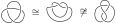
\includegraphics[width=.5\linewidth]{figures/intro/three-knots.pdf}
  \caption{Two equivalent knots and one inequivalent one}
\end{figure}
One of the central questions in knot theory is ``given diagrams $D_1$
and $D_2$ how do we determine whether they represent the same knot?''
If starting from first principles, this question is \textbf{HARD} to
approach mathematically; in fact it requires a bit of topological
knowledge to even formulate the question properly. Thankfully, in
practice we don't usually need to think about any of that because of a
theorem proven by \cite{Reidemeister1927Dec} and, independently,
\cite{Alexander1926}. In essence, they were able to show that two
``well-behaved'' diagrams\footnote{Again, we'll discuss what
  ``well-behaved'' means in great detail during
  \cref{chap:knots-and-knot-diagrams}, but it boils down to ``the
  string only crosses itself in an $X$ shape.''} $D_1, D_2$ represent
the same knot iff $D_1$ can be turned into $D_2$ by a sequence of the
following so-called \emph{Reidemeister moves:}
\begin{figure}[H]
  \centering
  \includegraphics[width=12cm]{figures/intro/rmoves.pdf}
\end{figure}
\noindent%
which are creatively referred to (in left-to-right order) as
``Reidemeister I,'' ``Reidemeister II,'' and ``Reidemeister III,''
respectively.\footnote{We also include another move, which allows us
  to bend the string arbitrarily as long as we don't introduce a
  crossing.} Note, while Reidemeister III might look complicated, it's
really just saying that we can move one strand between the crossing
formed by two other strands.

On a theoretical level, this is a very elegant characterization of
knot equivalence. However, in practice, determining equivalence is
still quite challenging. Even if $D_1$, $D_2$ are relatively simple
and both represent the same knot, the sequence of moves relating the
two can be quite long. It's even worse when $K_1 \not \cong K_2$,
because then we have to prove a negative result: namely, that there
\emph{does not exist} a sequence of Reidemeister moves takes $D_1$ to
$D_2$! Again, this is usually quite hard. Though Algorithms deciding
the problem do exist, they are currently far too inefficient to be
practical. For those who are familiar with Complexity Theory: It has
been proven (\cite{Hass1998Jul}) that a special case of knot equality
is at least NP. Reidemeister-based algorithms for the general problem
have runtimes like $O(k\uparrow\uparrow n)$ (\cite{Lackenby2016Apr}),
which makes even an NP solution seem out of reach for now.

% and current theoretical results {\color{red} IS THIS
%   TRUE? {\color{orange} put our best bound at EXPSPACE.}}


% It's a little baffling that these seemingly simple objects

But why? This seems like it should be easy! Our objects are very
tangible, the space we're working in ($\RR^3$) is well-behaved, and we
aren't asking for anything too fancy --- just a simple way to
determine equality. How can we understand the source of this
difficulty? Here, an analogy with something more familiar will be
helpful.






% ------------------------------------------------------------------ %
%                                                                    %
%                                2                                   %
%                                                                    %
% ------------------------------------------------------------------ %

\section{An Analogy}\label{sec:an-analogy}
Let's say I hand you two integers $n, m$. Would you be able to tell me
if $n = m$? Most likely the answer is yes. For instance, if I said
\begin{align*}
  n &= 8 & m &= 31
\end{align*}
you'd probably be able to distinguish $n$ and $m$. In particular,
they're uh\ldots not\ldots the same number.

But now let's frame the same problem in a slightly different way.
Suppose I had given you something like
\begin{align*}
  n &= ((1 + 3) + 3) + 1
  & m &= (((3 \cdot 3) \cdot 3) + (2 \cdot 2)) \cdot 1
\end{align*}
instead. Could you still determine if $n = m$? Maybe mental arithmetic
isn't your forte, but in theory the answer is ``yes'' --- these
equations give us the same solutions for $n,m$ as before, we just have
to do a little bit of extra work to see it.
% since the answers are obfuscated by a layer of arithmetic.
\begin{align*}
  n
  &= (4 + 3) + 1
  &
    m
  &= ((9 \cdot 3) + (2 \cdot 2)) \cdot 1 \\
  &= 7 + 1
  &
    m
  &= (27 + (2 \cdot 2)) \cdot 1 \\
  &= 8
  &
    m
    &= (27 + 4) \cdot 1
\end{align*}
For all intents and purposes these are cosmetic differences; they
don't make the problem too much harder to solve than it was before. We
can just simplify the expressions, see that the left gives $8$ and the
right gives $31$, and then we know $8 \neq 31$ so we can go on our
way.

This continues to hold even when the expressions get comically large,
e.g.
{\footnotesize
\begin{align*}
  n
  &= 2\cdot (2\cdot (8 \cdot  (21 - 38) - 7\cdot 6) + (4\cdot (21 +
    (-10 \cdot  (2 - 4))) + 7\cdot 28)) \\
  m &= (2\cdot(-3 \cdot (1500)) - 4) - (4\cdot(18-(8\cdot(10 - (3 -
      12)))))\cdot 15 + 5 \cdot(25\cdot(3\cdot4) - 101)
\end{align*}}
While simplifying these by hand might be tedious and unpleasant, it's
certainly something we could get a computer to do. In fact, programs
for this task are fairly efficient, being able to handle expressions
far larger than the above with near-instantaneous results.\footnote{To
  be precise: We claim we can verify equality of two $n$-bit integer
  arithmetic expressions in $O\pn{n \log^2(n)}$ time --- not too much
  worse than the $O(n)$ time for a direct equality check. We would
  like to acknowledge Jonathan Hayase for helping to produce the
  argument below.

  Sketch: First, note that given any two $k$-bit numbers, $+, -$ are
  $O(k)$ and $\times$ is $O(k \log k)$. Hence, without loss of
  generality the worst case for our problem is an input of the form $I
  = x_1 \times x_2 \times x_3 \times \cdots \times x_m$ where $m < n$
  and each of the $x_i$ are of the same length (requires some
  finagling to argue).

  Observe that multiplying two $k$-bit numbers yields (at most) a
  $2k$-bit integer. Hence, employing a divide-and-conquer approach, we
  can perform the total computation for $I$ recursively by computing
  $(x_1 \times x_2)$, $(x_3 \times x_4)$, \ldots, $(x_{m-1} \times
  x_m)$, and then using this to compute $((x_1 \times x_2) \times (x_3
  \times x_4))$, and so on. At the $\ell$\textsuperscript{th} pass, we
  multiply $2^{\log(n) - \ell}$ pairs of numbers, each of length
  $2^\ell$ bits, and there are $\log(n)$ passes total. This gives us a
  final runtime of $\sum_{\ell=1}^{\log(n)-1} 2^{\log(n) - \ell} \cdot
  2^{\ell} \log(2^\ell) = n \cdot \sum_{\ell=1}^{\log(n)-1} \ell = n
  \cdot \frac{\pn{\log(n) - 1} \cdot\log(n)}{2}$, which is $O(n
  \log^2(n))$.

  We run this algorithm twice (once for each side of the equation),
  and then finally check the resulting products for equality, which
  runs in $O(n)$. This gets us a total runtime of $O(n \log^2(n))$,
  which is quite fast.}

% Note, this approach continues to work
% even with extremely messy expressions like
% \begin{align*}
%   n
%   &= \frac{(154-162)\cdot(-\frac{66}{13})}{6} \cdot \frac{9}{29} -
%     \frac{38}{377} \\[1em]
%   m
%   &= \frac{\pn{\frac{7 + 90}{36 \cdot 5\cdot 5} + 8\cdot\frac{10}{764}}
%     \cdot \frac{1719}{1-54\cdot \frac{3\cdot 11 \cdot 3}{(63 + 37)
%     \cdot (35 + 19)}} - 3\cdot 9}{7300}.
% \end{align*}

The point of these examples is the following insight: When we say
things like ``$n=8, m=31$,'' we are often really thinking about
\emph{equivalence classes} of arithmetic expressions that can be
converted into each other using the standard rules of
algebra.\footnote{Recall, we denote the equivalence class of $x$ by
  $[x]$.} Hence, when we say things like
\[
  8 = ((1 + 3) + 3) + 1
\]
we really mean
\[
  8 \in [8] \qquad\text{ and }\qquad ((1 + 3) + 3) + 1 \in [8].
\]
In a deep sense, this is the same kind of problem we're tackling with
knots. We're given two ``expressions'' (knot diagrams) representing
our objects of interest, and we want to know whether they can be
converted into each other by a sequence of rules (Reidemeister moves)
that preserve equivalence. In this sense, Reidemeister moves can be
thought of as analogous to things like ``adding $0$ to both sides'' or
``rearranging terms.'' That is,
\[
  0 = 0 + (1 - 1)
\]
is philosophically similar to
\begin{figure}[H]
  \centering
  \includegraphics{figures/intro/add-one.pdf}
\end{figure}
Of course, the analogy isn't perfect. If it were, then we could just
import all of our techniques for simplifying expressions in $\ZZ$ to
the context of Knots and the problem would be solved! In the next
section, we'll scrutinize some of the differences that cause the
analogy to break down. Understanding exactly where we lose the
structure we rely on in $\ZZ$ will be essential in motivating the
questions we'll examine throughout the rest of this document. Hence,
we now turn our attention to these concerns.

\section{Where the Analogy Breaks Down}\label{sec:analogy-breakdown}
First we define some helpful vocabulary to make concepts like
``simplest form'' a bit more rigorous. Note, the terms below are
sometimes used with different meanings in different fields.
\begin{definition}[Normal Form]\label{def:normal-form}
  Let $S$ be a set of strings with an equivalence relation $\sim$ and
  a length function $\ell$.\footnote{$\ell$ just counts the number of
    symbols that appear in our written representation of elements of
    $S$. E.g., if the string $\texttt{123}\in S$, we'd have
    $\ell(\texttt{123}) = 3$.} Let $s \in S$. Then we say $s$ is in
  \emph{normal form} (also sometimes called \emph{simplest form}) if
  there exists no $s' \in S$ such that $s' \sim s$ and $\ell(s') <
  \ell(s)$.
\end{definition}
Basically, a normal form for some $s$ is the shortest possible
expression equivalent to $s$. In the integers, we'd say the string
\np{$1 + 1$} is not in normal form, as it requires $3$ characters to
write out (two numerals and a $+$ sign), while \np{$2$} only requires
$1$ character to write. For knots, one of the most natural choices for
$\ell$ is the number of crossings in the knot.

Note, we do not require normal forms to be unique; e.g., if we're
working with two-variable polynomial strings, then $x+y$ and $y+x$
would both be considered normal forms. They are equivalent under
$\sim$, but not identical as strings. We employ another definition
when we care about uniqueness: % {\color{blue} it seems like one of
  % these definitions should be removed.}
\begin{definition}[Canonical Form]\label{def:canonical-form}
  Let $S$ be a set of strings with an equivalence relation $\sim$.
  Index the equivalence classes of $S/\sim$ by some set $I$. For each
  $i \in I$, select a representative element $s_i$ from $[s]_i$. Then
  we say $s_i$ is the \emph{canonical form} for all $s \in [s]_i$.
\end{definition}
If one wants to think about canonical form more tangibly in terms of a
simplification process, the definition can be restated in terms of
functions:
\begin{definition}[Canonicalization]\label{def:canonicalization}
  Let $S$ be a set of strings with an equivalence relation $\sim$.
  Then a \emph{canonicalization} is a map $c : S \to S$ such that
  \begin{enumerate}
    \item For all $s \in S$, $c(c(s)) = c(s)$, and
    \item For all $s_1, s_2 \in S$, we have $s_1 \sim s_2 \iff c(s_1)
      = c(s_2)$.\qedhere
  \end{enumerate}
\end{definition}
The correspondence to \cref{def:canonical-form} comes with the
observation that for all $s$, $c(s)$ satisfies the requirements given
in \cref{def:canonical-form} for the canonical element of $[s]$.

Ok, now we turn to examining the differences between $\ZZ$ and knots.
There are two big ones we'll focus for now:
\begin{enumerate}[label=(\arabic*)]
  \item We have no efficient algorithm for reducing knot diagrams to
    normal forms using Reidemeister moves.\footnote{Here,
    ``simplifying'' means finding an equivalent diagram with fewer
    crossings.}
  \item What's more, even if there \emph{were} such an algorithm,
    it would not give us a canonical form. This is because normal
    forms for knots are not unique, in contrast to the situation in
    $\ZZ$ and $\QQ$.
\end{enumerate}
Let's expand on these points. Regarding (1): Note that when we
simplified our integer arithmetic expressions, each line had fewer
terms than the ones above. E.g.,
\begin{align*}
  m
  &= (((3 \cdot 3) \cdot 3) + (2\cdot 2)) \cdot 1 \\
  &= ((9 \cdot 3) + (2\cdot 2)) \cdot 1 \\
  &= (27 + (2\cdot 2)) \cdot 1 \\
  &= (27 + 4) \cdot 1 \\
  &= 31 \cdot 1 \\
  &= 31.
\end{align*}
That is, each step of the simplification process took us strictly
closer to a normal form. This is not an inherent property of
simplification algorithms in general. If, for instance, we were
working in arithmetic expressions over $\QQ$, then we could have
situations like the following:
\begin{align*}
  \ell
  &= \frac{1}{3} + \frac{1}{2}. \shortintertext{In order to simplify
    this expression symbolically, we actually have to make it more
    complicated first. In particular, making the terms share a common
    denominator requires adding extra symbols.}
  &= \frac{1 \cdot 2}{3 \cdot 2} + \frac{1}{2} \\
  &= \frac{1 \cdot 2}{3 \cdot 2} + \frac{1\cdot 3}{2\cdot 3}\\
  &= \frac{(1 \cdot 2) + (1 \cdot 3)}{3 \cdot 2} \\
  &= \frac{2 + (1 \cdot 3)}{3 \cdot 2} \\
  &= \frac{2 + 3}{3 \cdot 2} \\
  &= \frac{2 + 3}{6} \\
  &= \frac{5}{6}.
\end{align*}
We encounter a similar situation with Knots. Consider the following
example from \cite{Kauffman2011Sep}:
\begin{figure}[H]
  \centering
  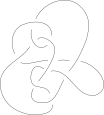
\includegraphics[scale=.3]{figures/intro/hard-unknot.pdf}
  \caption{A ``hard'' unknot}
\end{figure}
Although perhaps not immediately obvious, this is an unknot. To see
this, note that the strand going horizontally across the middle of the
knot can be pulled up behind the arc at the top, tucked down through
the same arc, and then out through the middle arc, at which point one
can apply a Reidemeister II move followed by a reidemeister I move to
undo the knot. For a more detailed view using only Reidemeister moves,
see \cite{Kauffman2011Sep}.

One can verify that there are no Reidemeister I or Reidemeister II
moves that we can perform without adding more crossings to the
diagram. What's more, there are actually \emph{no} Reidemeister III
moves available at all. Thus, this is a knot diagram that has to be
made more complicated before it can be reduced, similarly to the
fractions in $\QQ$.

However, there is a key distinction between these two cases. With the
fractions in $\QQ$, it's always fairly obvious what the next step
should be. We scan left-to-right looking for two fully-simplified
sub-expressions we can combine together; if they're both fractions,
then we convert everything to a common denominator. Next, we combine
the numerators, and then finally we simplify. While seemingly not as
efficient as parsing arithmetic expressions in $\ZZ$, we can still
develop a {greedy algorithm} to attack the problem.

By contrast, there seems to be no obvious strategy to determine which
strands we should move first on the unknot shown above --- or at
least, there isn't one that scales well to large knots.\footnote{This
  doesn't mean one does not exist --- but to the author's knowledge,
  nobody has found one yet.} Hence the simplification problem for
knots seems a bit ``harder.''

Now, regarding (2) (``even if there were such a simplification
algorithm, this still wouldn't immediately give us a canonical
representative.''). The problem here is that in $\ZZ$ and $\QQ$, the
normal forms yielded by our simplification algorithms ended up
coinciding with our canonical forms. Thus, after simplifying
completely, we could simply check for literal equality. This is not
always the case with Knots.%  {\color{blue} We will give a more general
  % strategy for constructing counterexamples later, but the idea is
  % something like this:}
\begin{figure}[H]
  \centering
  \includegraphics[scale=.6]{figures/fundamentals/sum-at-0.pdf}
\end{figure}
\begin{figure}[H]
  \centering
  \includegraphics[scale=.6]{figures/fundamentals/sum-at-3.pdf}
  \caption{Two drawings of the same knot.}
\end{figure}
The reader can verify that these diagrams contain the same number of
crossings. It is harder to see why they are equivalent, though the way
we've drawn them might be suggestive of an argument.\footnote{If the
  reader would like to give this a shot, we heavily encourage a more
  hand-wavey proof that does \emph{not} attempt to employ the
  Reidemeister moves.} It is known that the diagrams above are in
normal form (in that they achieve the minimal crossing number),
although we will not discuss the details in this document.
% {\color{blue} Really I'm just assuming the connected sum crossing
% conjecture and figuring that if this were a counterexample it'd be
% known already.}
In any case, we see that for knots, \np{normal form}
$\nRightarrow$ \np{canonical form}.

Taken in tandem, these problems make approaching the knot equivalence
problem quite challenging. However, there's one saving grace: if we
only want coarse, back-of-the-envelope heuristics for determining
whether two knots are ``probably'' equivalent, then we can actually
employ strategies similar to those used in $\ZZ, \QQ$. This is the
motivation for \emph{invariants.}

\section{Invariants, Briefly.}\label{sec:invariants-briefly}
Hey you --- {\bfseries Think fast!} In 10 seconds or less, which of
the following are true?\footnote{\ldots I'm counting.}
\begin{leftbar}
  \begin{enumerate}[leftmargin=2em]
      \small
    \item $5\pn{3^3 \cdot 11}^2 = 2 (72 + 33 - 8)$
    \item $\displaystyle -\frac{2}{\pn{\sqrt{47} +
      \frac{1}{47}}^{3}} = 47 - \frac{1}{47^2}$
    \item $\displaystyle 3x^4 + (x + 3)(x^2 + 2x + 2) +
      \frac{2}{3}(x - x^2) = 2\pn{x^4 + \frac{3}{2}x(x^2 - 3x)} +
      3x$
  \end{enumerate}
\end{leftbar}
Ok, hopefully that was far too little time to actually figure them all
out. As it turns out, they are all false. Here are some short
arguments for why:
\begin{leftbar}
  \begin{enumerate}
    \item Note that all the factors on the left side ($5$, $3$, $11$)
      are odd, while the right has a leading factor of $2$. So they're
      not equal.
    \item Observe that the left side is negative, while the right side
      is positive (since $47 > 1 > \frac{1}{47^2}$).
    \item This one takes more time to verify, but the leading
      coefficients don't match ($3$ and $2$, respectively). Also, the
      right side has no constant term, whereas the left side does.
  \end{enumerate}
\end{leftbar}
Implicitly, each of these are using an \emph{invariant} of arithmetic
strings. For 1., we know that if two expressions are equal, then if
one is even, the other must be even too. For 2., we are using the fact
that equivalent expressions must have the same sign. And for 3., we
use an invariant of polynomials --- namely that when simplified, their
coefficients must match up.

We can define similar invariants for many other problems. It's worth
noting that these don't always look like simple arithmetic properties,
as demonstrated by the following example:
\begin{example}\renewcommand{\qedsymbol}{}\label{ex:chessboard}
  Consider a $7\times 7$ chessboard with a knight placed on each
  square. Is there a way to move each night exactly once such that
  after each knight has been moved, no knight has left the board, and
  no knights have doubled up on the same square?
  \begin{figure}[H]
    \centering
    \includegraphics[scale=.75]{figures/fundamentals/chessboard.pdf}
    \caption{Diagram of the Situation}  % \qedhere
  \end{figure}
\end{example}
There is an extremely short solution. To emphasize just \emph{how}
short, we've included a redacted version of a short proof by one J.\
Yossarian, just to taunt the reader (an unredacted version can be
found in \cref{sol:chessboard}, \cpageref{sol:chessboard})
\begin{leftbar}
  \emph{Claim:} \censor{No.}\\

  \noindent \emph{Proof:} \censor{Observe that there} are \censor{25
    black squares} and \censor{24 white squares}. \censor{Also}
  \censor{note that every legal move takes} a \censor{knight to} an
  \censor{opposite-color square}. \censor{Hence} \censor{after moving
    all} the \censor{knights}, \censor{we}'\censor{d have 25 on black}
  and \censor{24 on white}, \censor{which is} a
  \censor{contradiction}. \hfill \censor{$\jiong$}
\end{leftbar}
Likewise, many of the invariants we employ in Knot Theory are hard to
connect to explicit algebraic structures we understand. Here are some
high-level examples --- we won't be studying invariants directly, so
don't worry too much about the details, the point is just to know that
they exist.
\begin{example}[Biquandles]
  Let $X$ be a set and $K$ be a knot represented by some diagram $D$.
  Label (``color'') each arc in $D$ by an element of $X$. Then, define
  two binary operations $\underop, \overop$ (read ``under'' and
  ``over,'' respectively) that describe how our labels change when
  strands cross.\footnote{Technically the words here are in the wrong
    order --- we aren't actually guaranteed that such operations exist
    if we begin with an \emph{arbitrary} coloring. But this is meant
    to capture the high-level overview of what the biquandle axioms
    seek to do, so we'll leave it like this for today.}
  \begin{figure}[H]
    \centering
    \includegraphics[scale=.7]{figures/fundamentals/biquandles.pdf}
    \caption{Example of a colored crossing}
  \end{figure}
  By translating the Reidemeister moves into algebraic axioms for
  $\underop, \overop$, we can turn ``coloring by $X$'' into a knot
  invariant:\footnote{The biquandle axioms can look somewhat
    intimidating at first, but with the right diagrams, one can see
    that they are direct translations of the reidemeister moves. We
    haven't included such diagrams since again, we won't really be
    working with biquandles, but for more we encourage the reader to
    reference \cite{NelsonBook}, which we found to be an excellent
    resource.}
  \begin{enumerate}
    \item For all $x \in X$, $x \underop x = x \overop x$,
    \item For all $x,y \in X$, the maps $\alpha_y, \beta_y : X \to X$
      and $S : X \times X \to X \times X$ defined by
      \[
      \alpha_y(x) = x \overop y, \quad \beta_y(x) = x \overop y \quad
      \text{and} \quad S(x,y) = (y \overop x, x \underop y)
      \]
      are all invertible, and
    \item For all $x,y,z \in X$, we have the following \emph{exchange
      laws}:
      \begin{align*}
        (x \underop y) \underop (z \underop y)
        &= (x \underop z) \underop (y \overop z) \\
        (x \underop y) \overop (z \underop y)
        &= (x \overop z) \underop (y \overop z) \\
        (x \overop y) \overop (z \overop y)
        &= (x \overop z) \overop (y \underop z)
      \end{align*}
  \end{enumerate}
  In this case we call $(X, \underop, \overop)$ a \emph{biquandle}.
\end{example}
Biquandles are an example of \emph{coloring invariants}, which are
currently a popular area of study. Another example of a well-known
class of knot invariants is the family of \emph{knot polynomials}.
Knot polynomials are generally agreed to be some of our most powerful
invariants, combining ease of computation with relatively good
performance in distinguishing between knots. An example is the
celebrated \emph{Jones polynomial}, which can be recursively computed
from a knot diagram using the \emph{Kauffman Bracket}:
\begin{example}[Jones Polynomial]
  Define a map $\bk{\ }$ on formal sums of knot diagrams as follows:
  \begin{figure}[H]
    \centering
    \includegraphics[scale=.55]{figures/fundamentals/jones-polynomial.pdf}
    \caption{Kauffman Bracket}
  \end{figure}
  where the diagram is unchanged outside of the dotted neighborhood.
  After applying the bracket map until there are no crossings
  remaining, we're left with a formal sum whose terms are diagrams of
  some number of unlinked unknots. For each such term, apply the
  following conversion:
  \begin{figure}[H]
    \centering
    \includegraphics[scale=1]{figures/fundamentals/jones-delta.pdf}
    \caption{Converting unknots to polynomial terms}
  \end{figure}
  Now every term is a Laurent polynomial in $x$. Combine them all and
  and simplify to yield the \emph{Jones} polynomial.\footnote{This
    process is easier to follow by looking at some examples; the
    reader is encouraged to do so. This is also covered in
    \cite{NelsonBook}; an approach that combines knot polynomials
    \emph{with} coloring invariants like biquandles can be seen in
    \cite{Nelson2017Feb}.}
\end{example}
The Jones Polynomial has many remarkable properties; the reader is
encouraged to poke around through some of the literature on it.

\subsection{Fantastic Invariants \& Where to Find Them}
The section above is meant to highlight two main points: First,
invariants are helpful. We did not discuss explicit performance
metrics, but it is safe to say that employing them is generally much
easier than doing a brute-force search with Reidmeister moves. Second,
powerful invariants can look very different from each other.
Biquandles and the Jones polynomial both operate on diagrams, but do
so through very different mechanisms. This can make it tricky to
identify where we should look \emph{next} for new invariants, since it
can be hard to interpret exactly what structure they are preserving.
What other strategies can we try?

There are two main ways to approach this problem. First, we can try
and generalize the strategies that we know work to see if we can get
modified versions that perform better. A lot of interesting work goes
on here currently, including some of our own results on more general
methods for combining coloring invariants with knot polynomials
(\cite{Kobayashi2019Sep}). However, there is also a more direct
strategy---if we can find ways to describe algebraic structure in the
Knot category more explicitly, we might be able to understand
invariants from a more functorial perspective. Currently, this is
generally avoided, since the structure of the Knot category is not
very well-understood. However, there is one interesting approach that
has yielded some preliminary results recently, which is to make use of
unknotting moves.

Unknotting moves are operations on a diagram that can be used to
reduce arbitrary knots to the circle (an example is being allowed to
``flip'' which strand is on top at any given crossing). Observe that
for an arbitrary knot $K$, playing a sequence of unknotting moves for
$K$ in reverse gives us a way to create $K$ out of an unknotted
circle. Hence, there is a sense in which unknotting moves encode the
information of how to build a knot, and so it seems plausible that
examining them could give us insights into our invariants.

The literature contains precedent for this idea; for instance, it has
been shown that an unknotting move called the \emph{delta move}
affects some polynomial invariants in predictable ways (see
\cite{Kanenobu2005Jan}, \cite{Ganzell2014Feb}). However, there has
been little analysis of the effects of other kinds of unknotting
moves, the effects of performing multiple moves in succession, and
whether the results found can be generalized to other kinds of
invariants. So, in general, the idea remains largely unexplored.

Our motivating goal for this project was to try and attack the problem
of using unknotting moves to define a group-like structure on knots.
The hope is that if we can do so, it will make it easier to search for
powerful invariants by looking at something more homomorphism
flavored.


% As discussed in the overview, pursuing this idea


% and see if tuning some parameters can get us stronger
% results.\footnote{This makes it sound a lot less impressive than it
%   is! Lots of interesting work goes on here.}




%%% Local Variables:
%%% TeX-master: "../../kobayashi-thesis"
%%% End:
